\section{Introduction}

Thermal reflow can significantly modify the profile of structures obtained in polymer resist and this phenomenon has its advantages and disadvantages.
For example, thermal reflow could be used for smoothing of the relief obtained by grayscale e-beam lithography~\cite{Kirchner_GL_review} which allows to obtain various 3D structures.
On the other hand, thermal reflow leads to relief deformation, which is undesirable in certain cases~\cite{NIL_reflow}.
In the light of the above, the method allowing exact determination of thermal reflow influence on resulting structure profile in any specific processes is highly desirable.

Two common approaches to thermal reflow simulation of polymer structures could be distinguished.
The first include analytical methods based on transfer equations.
For instance, Leveder~\cite{Leveder_2010,Leveder_2011} used an analytical spectral method to simulate the reflow of periodic structures obtained in polystyrene by nanoimprint lithography.
This method is based on two-dimensional Navier-Stokes equation coupled to continuity equation  considering Laplace pressure and Hamaker energy with the assumption of no slip length and no Marangoni effect.
In this method the initial structure profile undergoes Fourier transform and then thermal reflow is being simulated by decay of profile harmonic modes:
\begin{equation} \label{eq:Fourier_1}
	h(x, t) = h_0 + \tilde{h}(x, t),
\end{equation}
\begin{equation} \label{eq:Fourier_2}
	\tilde{h}(x, t) = \sum_{-\infty}^{+\infty} a_n(0) \exp \left(-\frac{t}{\tau_n}+i n \frac{2 \pi}{\lambda} x \right),
\end{equation}
\begin{equation} \label{eq:Fourier_3}
	\tau_n = \frac{3 \eta}{\gamma h_0^3} \times \left( \frac{\lambda}{2 \pi n} \right)^4,
\end{equation}
where $\lambda$ -- profile spatial periodicity, $\eta$, $\gamma$ -- polymer viscosity and surface tension, respectively, $a_n(0)$ -- Fourier coefficients of initial polymer profile, $h_0$ -- polymer layer thickness.
Polymer viscosity depends both on temperature and polymer molecular weight, which should be taken into account.
Temperature dependence of viscosity could be described by Williams–Landel–Ferry (WLF) equation~\cite{Bird_WLF}:
\begin{equation} \label{eq:WLF}
	\log \left( \frac{\eta(T)}{\eta(T_0)} \right) = -\frac{C_1(T-T_0)}{C_2+(T-T_0)},
\end{equation}
which parameters $\eta(T_0)$, $C_1$, $C_2$ and $T_0$ for three different polymers are provided in Table~\ref{table:WLF}~\cite{Aho_WLF}.
The dependence of polymer viscosity on its molecular weight could be described by empirical formula:

\begin{equation} \label{eq:3p4_3p1}
	\eta \propto M_n^\alpha,
\end{equation}
where $M_n$ -- number average polymer molecular weight. For polymethyl methacrylate (PMMA) $\alpha$ comprises 3.4 at $M_n > 48000$ and 1.4 at $M_n < 48000$~\cite{Leveder_2010,Bueche_3p4_1p4}.
Equations~\ref{eq:WLF}, and \ref{eq:3p4_3p1} allow one to calculate polymer viscosity for different temperatures and values of number average molecular weight (Fig.~\ref{fig:eta_vary_T_Mn}).

\begin{figure}
	\begin{center}
		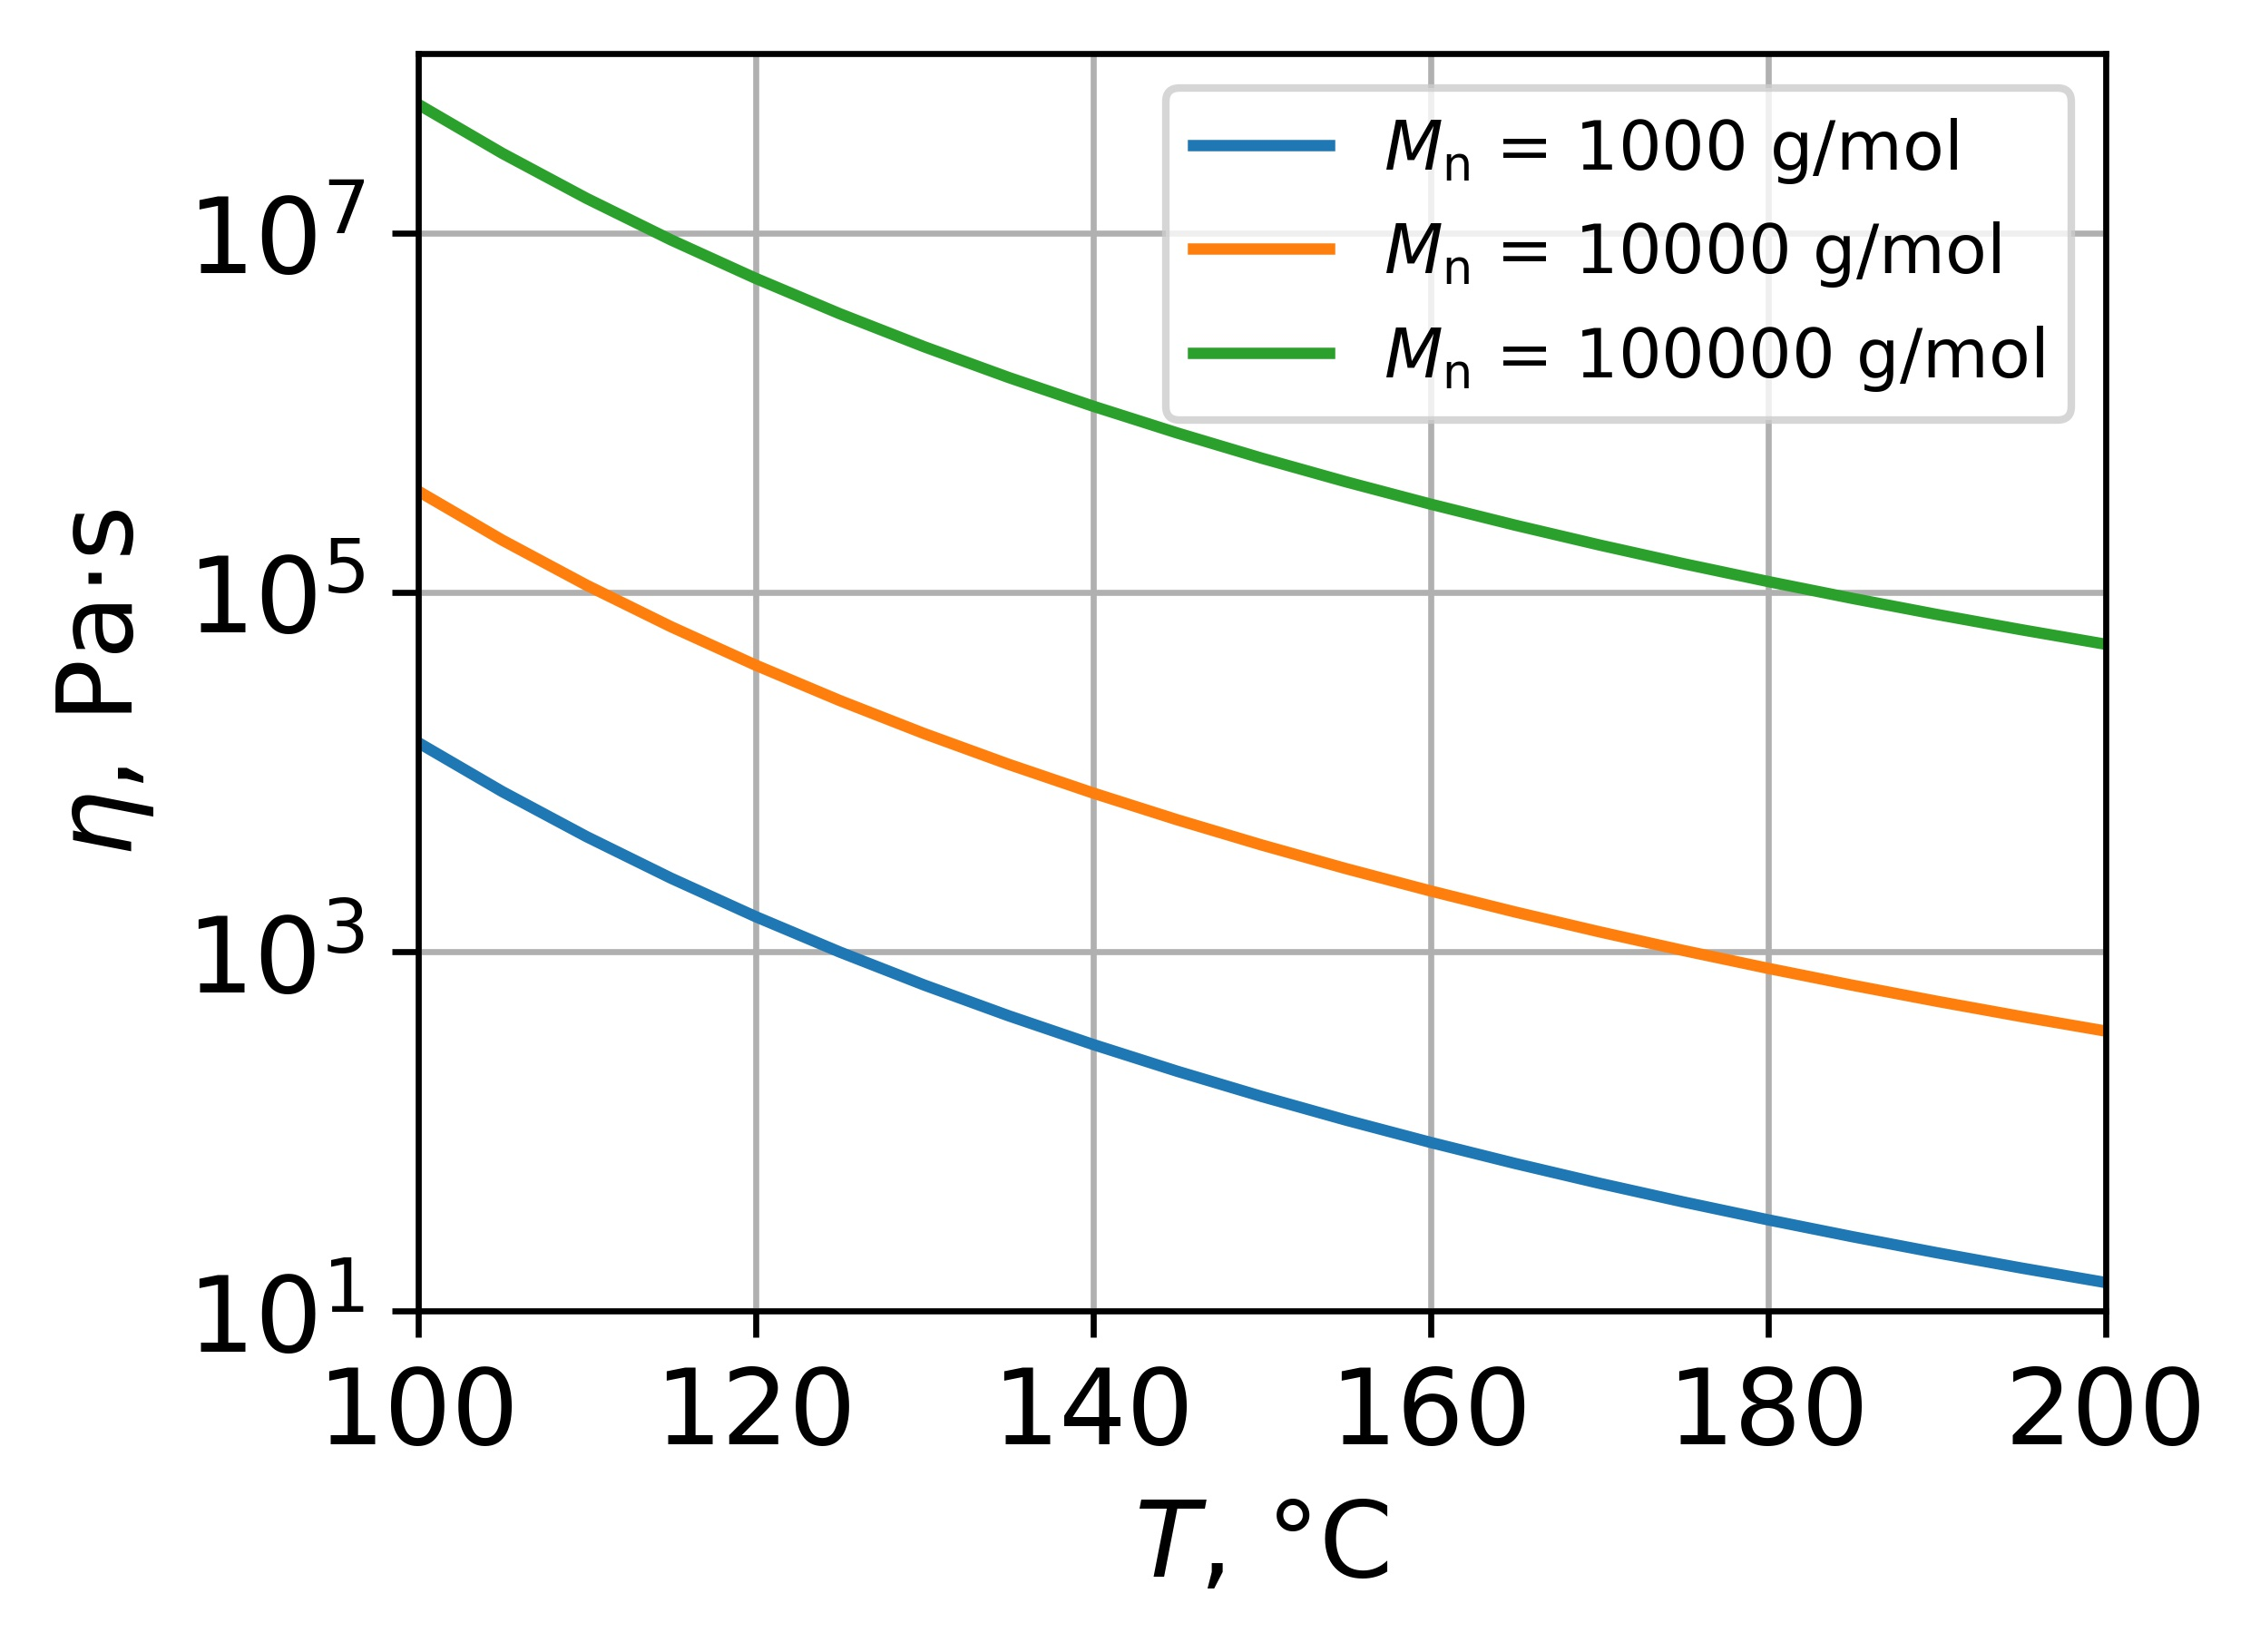
\includegraphics[width=0.6\linewidth]{eta_vary_T_Mn}
	\end{center}
	\vspace{-2em}
	\caption{Temperature viscosity dependencies for PMMA with different number average molecular weights, obtained by equations~(\ref{eq:WLF}, \ref{eq:3p4_3p1}).}
	\label{fig:eta_vary_T_Mn}
\end{figure}

\begin{table}[t]
	\centering
	\caption{Parameters of equation~\ref{eq:WLF}, obtained by Aho et al. for polystyrene 143E by BASF (PS), polymethyl methacrylate Plexiglas 6N by Degussa (PMMA) and polycarbonate Lexan HF1110R by GE Plastics (PC)~\cite{Aho_WLF}.}
	\begin{tabular}{@{}llll}
		\br
		Parameter \hspace{8.9em} & PS \hspace{5em} & PMMA \hspace{5em} & PC \\
		\mr
		$\eta(T_0)$, Pa$\cdot$s \hspace{8.9em} & 7310.4 \hspace{5em} & 13450 \hspace{5em} & 2763 \\
		$C_1$ \hspace{8.9em} & 10.768 \hspace{5em} & 7.6682 \hspace{5em} & 4.7501 \\
		$C_2$, $^\circ$C \hspace{8.9em} & 289.21 \hspace{5em} & 210.76 \hspace{5em} & 110.12 \\
		$T_0$, $^\circ$C \hspace{8.9em} & 190 \hspace{5em} & 200 \hspace{5em} & 200 \\
		\br
	\end{tabular}
	\label{table:WLF}
\end{table}

The second approach, numerical one, is based on search of minimal surface by finite elements method. It can be processed by free software ``Surface Evolver'' (SE) -- the program for the modelling of liquid surfaces shaped by various forces and constraints~\cite{Brakke_SE}. SE allows a wide spectrum of possible energies to be assigned like gravitational energy, surface energy, and further different implementations of mean and Gaussian curvature. For the purpose of polymer reflow simulation only surface energy should be taken into account.

In SE simulation algorithm the structure is only described by its ``outer shell'' (soapfilm modeling)~(Fig.~\ref{fig:SE_basic}a). The resist surface is being divided into triangle facets defined by vertices $v_0$, $v_1$ and $v_2$ and oriented edges $\vec{e_0}$, $\vec{e_1}$ and $\vec{e_2}$, and the polymer reflow is simulated by moving of facet vertices, maintaining the constant volume inside the surface. The force on vertex $v_0$ (the tail of vector $\vec{e_0}$) is

\begin{equation}
	\vec{F}_{v_0}=\frac{\gamma_i}{2} \cdot \frac{\vec{e}_1 \times\left(\vec{e}_0 \times \vec{e}_1\right)}{\left\|\vec{e}_0 \times \vec{e}_1\right\|},
\end{equation}
where $\gamma_i$ -- is surface tension of $i$-th facet~(Fig.~\ref{fig:SE_basic}b). SE could be operated in the area normalization mode to approximate a vertex motion by mean curvature, i.e., a surface tension flow. In this mode, the velocity of a vertex is proportional to force and indirectly proportional to the area of the facets surrounding this vertex. The $i$-th facet has three vertices associated with it, therefore the relative area contribution to the force of one vertex is 1/3 the area of the surrounding facets $A$. The vertex velocity in the area normalization mode is

\begin{equation} \label{eq:SE_v}
	\vec{v} = \frac{\vec{F}}{A/3} \cdot \mu,
\end{equation}
where $\mu$ is so called vertex mobility. The vector of vertex movement $\vec{\delta}$ is then calculated as product of vertex velocity and \textit{scale} factor, the physical representation of simulation step time:

\begin{equation} \label{eq:SE_delta}
	\vec{\delta} = \vec{v} \cdot scale.
\end{equation}
In most cases SE is used for calculation of minimal energy geometries only~\cite{SE_example_1,SE_example_2}, which doesn't imply simulation of liquid or polymer flow dynamics.

\begin{figure}[t]
	\centering
	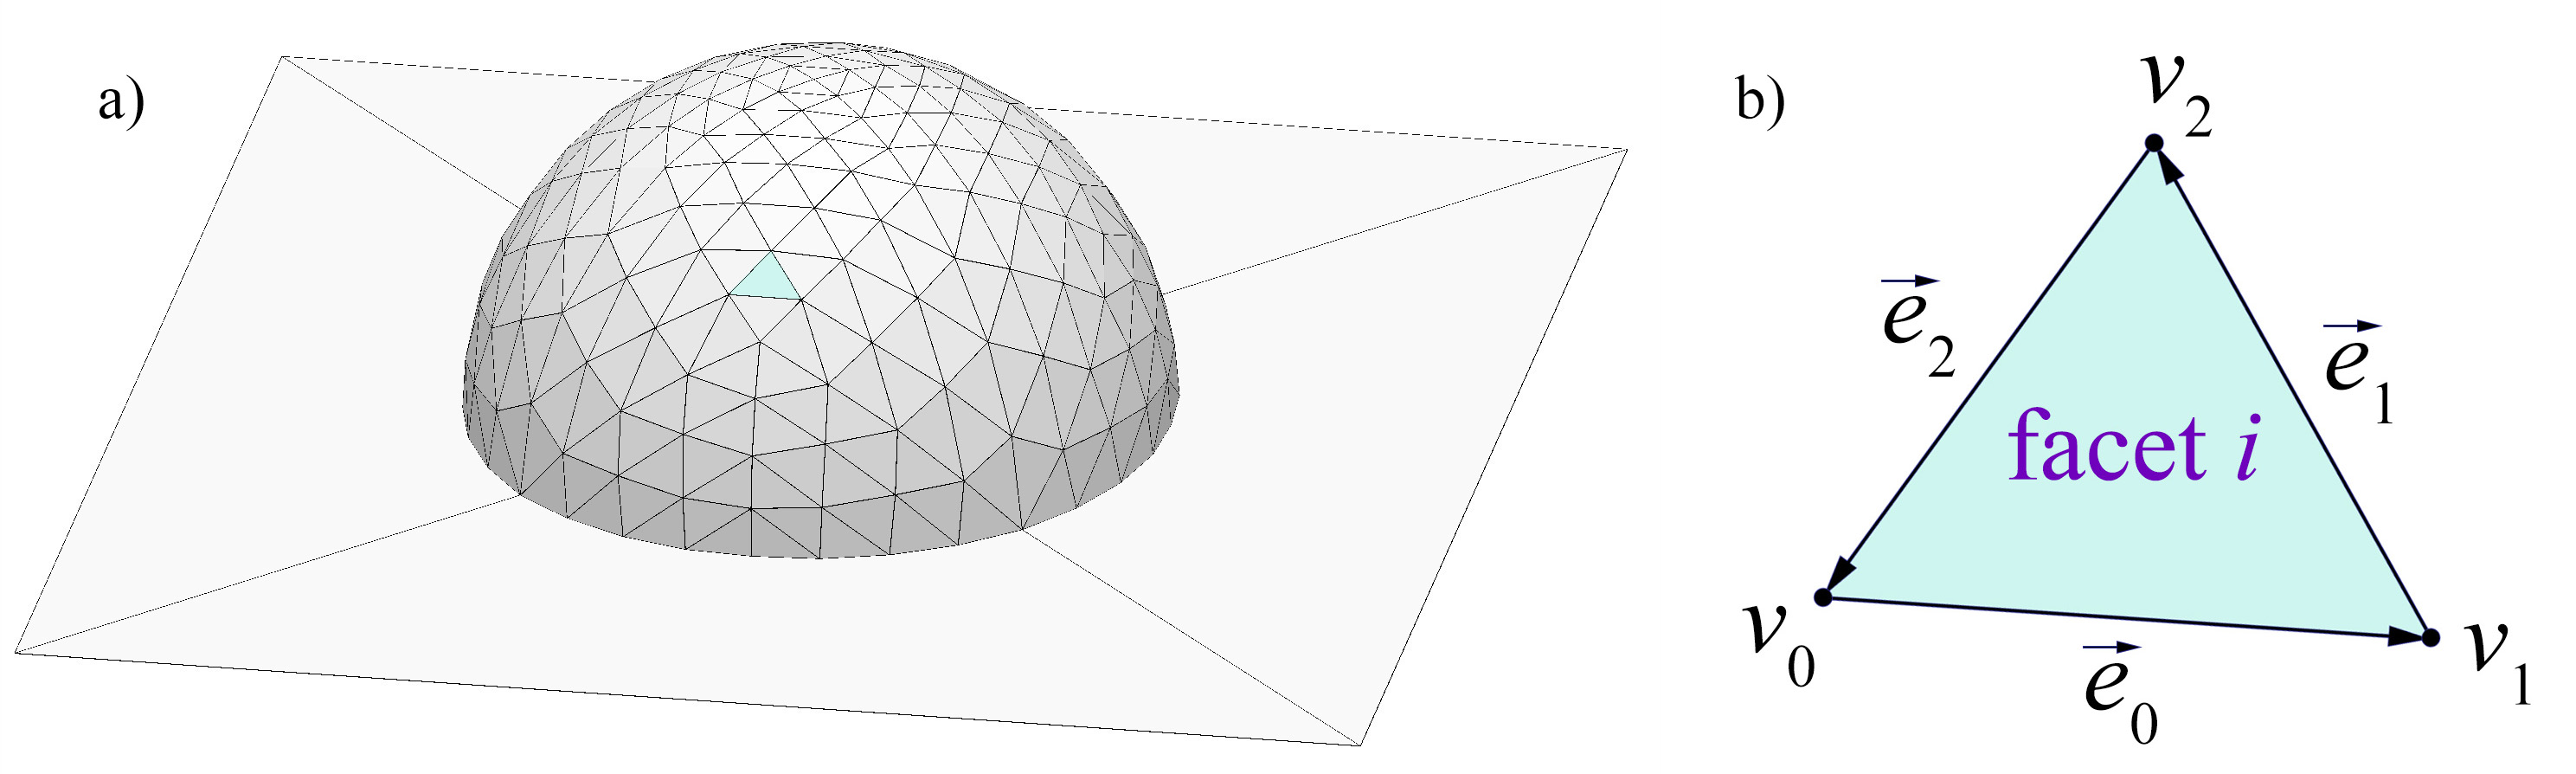
\includegraphics[width=\linewidth]{Fig_2} \\
	\caption{a) A mound of liquid sitting on a tabletop with gravity acting on it, defined by its surface in SE, b) definition of vertices and oriented edges for $i$-th facet in SE.}
	\label{fig:SE_basic}
\end{figure}

Polymer structures obtained by grayscale e-beam lithography have strongly non-uniform distribution on number average molecular weight, which result in non-uniform viscosity profile.
Analytical spectral approach could not be applicated in this case, but numerical one can still be used.
Kirhner~\cite{Kirchner_SE_1} applied SE for thermal reflow simulation of double-step structures obtained in PMMA by e-beam grayscale patterning and wet development.
The structures consisted of two regions with different values of PMMA number average molecular weight, and the difference in region viscosity was taken into account by setting different vertex mobilities.
Mobility ratios for structure regions were determined empirically by the comparison of simulated profiles to the experimental ones.
In this case, the simulation algorithm is only applicable for the structures obtained with the same exposure doses, and reflow simulation of any other structure requires preliminary measurements.
On the other hand, in case of any structure reflow simulation, carried out using SE, the only question is the distribution of structure vertex mobilities.
Kirchner mentioned that inverse mobility should correlate with PMMA viscosity, but the relation between mobility and viscosity was still unclear.
%Thus, the purpose of this study is to investigate the relation between polymer viscosity and mobility of its surface vertices and to develop the numerical approach for thermal reflow simulation of non-uniform polymer structures obtained by grayscale e-beam lithography using SE as a calculation engine.
Thus, the aim of this study is to develop the numerical approach for thermal reflow simulation of non-uniform PMMA structures obtained by grayscale e-beam lithography using SE as a calculation engine.
For this purpose one should simulate viscosity profile of e-beam exposed PMMA first and then
investigate the relation between PMMA viscosity and mobility of its surface vertices.
